\chapter{Inleiding}
\label{ch:introduction}

Dit verslag is geschreven in opdracht van de Hogeschool van Arnhem in Nijmegen
(HAN) in het kader van de minor Embedded Vision Design (EVD) aan de opleiding
Embedded Systems Engineering (ESE). Het omschrijft hoe het project van de studenten
is ontwikkeld en waarom bepaalde design keuzes zijn gemaakt gedurende de
ontwikkeling van het product.

Het doel van het project was om een autonome \emph{Nerfgun} (zie figuur \ref{fig:nerf})
te ontwikkelen. Dit product moet in staat zijn om een persoon te herkenning
en er vervolgens een \emph{dart} (figuur \ref{fig:nerfdart}) op af te vuren. De
officiele omschrijving van het project is als volgt:

\begin{quote}
“Uiterlijk week 8 van het academisch jaar 2013/2014 zal een systeem ontwikkeld zijn die
autonoom een Nerfgun kan afvuren op bewegende doelwitten (personen). Het systeem moet
gebruik maken van camera beelden om deze doelwitten te vinden binnen een omgeving.”
\end{quote}

Het systeem is gedoopt tot \emph{Autonerf} (een samenvoeging van \emph{autonoom}
en \emph{Nerf}). In dit verslag worden de resultaten van de verschillende projectfasen besproken
en uitgelegd.

\vfill
\pagebreak

Het eerste deel dat zal worden beschreven is het functioneel ontwerp
(\ref{ch:functional}). Hier zal functioneel beschreven worden \emph{wat} het
systeem moet doen. Er zal verder niet worden ingegaan op \emph{hoe} het systeem
dit bereikt. Het hoofdstuk Technische Specificatie (\ref{ch:technical}) zal hier
verder op ingaan. In hoofdstuk \ref{ch:realization} zal de realisatie van het
project beschrijven. Er zal besproken worden welke beslissingen er gemaakt zijn
en waarom deze gemaakt zijn. Uiteindelijk zullen de resultaten van het testen
(hoofdstuk \ref{ch:testing}) besproken worden. Daarnaast zal in hoofdstuk
\ref{ch:conclusion} een conclusie worden getrokken en zullen eventuele
aanbevelingen worden gedaan voor het doorontwikkelen van het product.

\begin{figure}[H]
    \begin{minipage}{0.45\textwidth}
        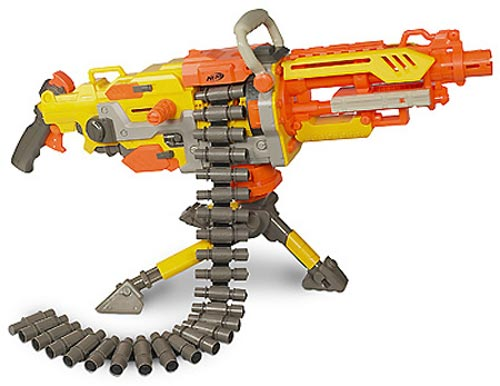
\includegraphics[width=\linewidth]{figures/nerfgun.jpg}
        \caption{Een Nerfgun}
        \label{fig:nerf}
    \end{minipage}
    \begin{minipage}{0.45\textwidth}
        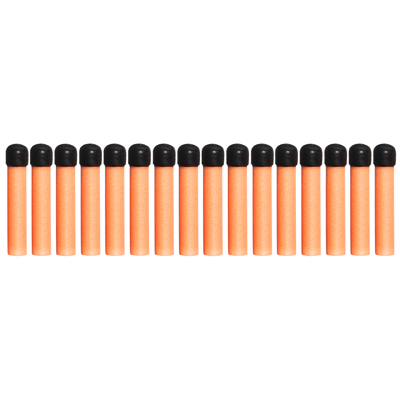
\includegraphics[scale=.5,width=\linewidth]{figures/nerfdart.png}
        \caption{Een Nerf dart}
        \label{fig:nerfdart}
    \end{minipage}
\end{figure}
